	\documentclass[12pt]{article}
	\usepackage{hyperref}
	\usepackage{graphicx}
	\usepackage[T1]{fontenc}
	\usepackage[utf8]{inputenc}
	\usepackage{color}
	\usepackage[font=small,labelfont=bf]{caption}
	\usepackage[english]{babel}
	\usepackage{datetime}
	\usepackage{fancyhdr}
	\usepackage{lastpage}
	\usepackage{float}
	\pagestyle{fancy}
	\fancyhf{}
	\usepackage{multicol}
	\rfoot{\center Page \thepage \hspace{1pt} of \pageref{LastPage}}
	\renewcommand{\today}{\thisdayofweekname\ \the\day\ \monthname\ \the\year}
	\title{Essay}
	\date{}
	\author{Trevisan Davide}
	\hypersetup{
		colorlinks=true,       % false: boxed links; true: colored links
		linkcolor=blue,          % color of internal links (change box color with linkbordercolor)
		citecolor=green,        % color of links to bibliography
		filecolor=blue,      % color of file links
		urlcolor=red,
		filecolor=red,
		citecolor=red,
	}
	\begin{document}
		\pagenumbering{arabic}
		
		
		
		\begin{titlepage}
			
			\newcommand{\HRule}{\rule{\linewidth}{0.5mm}} % Defines a new command for the horizontal lines, change thickness here
			
			\center % Center everything on the page
			
			%----------------------------------------------------------------------------------------
			%	HEADING SECTIONS
			%----------------------------------------------------------------------------------------
			
			\textsc{\LARGE University of Padova}\\[1.5cm] % Name of your university/college
			\textsc{\Large Computer and Network Security}\\[0.5cm] % Major heading such as course name
			
			%----------------------------------------------------------------------------------------
			%	TITLE SECTION
			%----------------------------------------------------------------------------------------
			
			\HRule \\[0.4cm]
			{ \huge insert-title-here}\\[0.3cm]
			 %TODO insert title 
			%Title of your document
			\HRule \\[1.5cm]
			
			%----------------------------------------------------------------------------------------
			%	AUTHOR SECTION
			%----------------------------------------------------------------------------------------
			
			\begin{minipage}{0.4\textwidth}
				\begin{flushleft} \large
					\emph{Students:}\\
					Davide Trevisan\\ % Your name
					Andrea Multineddu\\
				\end{flushleft}
			\end{minipage}
			~
			\begin{minipage}{0.4\textwidth}
				\begin{flushright}\large
					\emph{Registration number:} \\
					\textsc{1070686}\\ % matricola
					\textsc{matricola}\\
				\end{flushright}
			\end{minipage}\\[1cm]
			
			%----------------------------------------------------------------------------------------
			%	DATE SECTION
			%----------------------------------------------------------------------------------------
			
			{\large \today}\\[1cm] % Date, change the \today to a set date if you want to be precise
			
			%----------------------------------------------------------------------------------------
			%	LOGO SECTION
			%----------------------------------------------------------------------------------------
			
			
\includegraphics[scale=0.20]{Logo.png} % Include a department/university logo - this will require the graphicx package
			
			%----------------------------------------------------------------------------------------
			
			\vfill % Fill the rest of the page with whitespace
		\end{titlepage}
		
		\newpage

\begin{multicols}{2}
\section{Stealth Screenshot Extension}
The source code of the extension we developed is downloadable \href{URL}{here}
\subsection{Scope of the extension}
the scope of the stealth screenshot extension is to create a small prototype of an extension that catch screenshot in a regular interval with the minimum possible user interaction and obviously giving it back.
\subsection{How the extension work}
\subsubsection{Activation and screenshot collection}
The extension uses the relatively new tab APIs given by chrome too take screenshot.
The extension makes use of the "storage", "tabs", "all\_urls;", "unlimitedStorage", "activeTab" permissions in his manifest file. The extension works in a simple way: it triggers on a browser event, in this case the click on the icon of the extension, but there are other possibilities: we tested that there are no simple ways to take screenshot without no interaction, because the security policy of the API doesn't allow to take a scrrenshot without some kind of events, presuming that the user should be aware of what is happening; not triggering any event returns only null.
Once triggered, the extension schedule all the future screenshot through the Javascript setTimeout method: this allows to take screenshot for hours, with only the need for a click to start.
The screenshot are stored in an array visible to all the extention methods.
\subsubsection{Screenshot retrival}
The screenshot can be collected in two ways in the wxtension we developed:
through a combination of key for retriving all screenshots (we programmed it on Ctrl+Shift+Y) or writing "show" in the omnibox, pressing "tab" and writing in the omnibox the number of screenshot to show (starting from the last one).
\subsubsection{Performance}
We tested that the extension is able to take screenshot with a interval of 1 minute for more than 2 hours without losing any screenshot.
The application occupy less of 50MB of RAM for an hour of screenshots taken every minute. The impact on the CPU is negligible.
Screenshot retrival through the kay combo however can  crash chrome, although it never happened in our PC because of the great performance (we had an Intel i5 6400, with 8GB of DDR4 memory and SSD), but it got freezed for some seconds.
\subsection{Limitations}
The major limitation of this extension is that the screenshot only lives until the extension is active: this implies that closing all the windows of chrome completely deletes the screenshot taken.
This is a consequence of how the API and the chrome sandbox works. We at the moment found no way to get around it, but we are pretty confident that is possible to save those screenshots, but for our lack of knowledge we are not able at the moment to demonstrate it.
\subsection{Future work}
Possible future works will focus on find a way to save those screenshot.
The application should also be rewritten without the tab API, to avoid of the limitation of it.
Javascript inject the code for the screenshot or use it for simulate the right events should do the work, but the time and the train needed to do it made impossible for us to test it for this paper.
\section{conclusions}
All the solution we have presented in thispaper makes use of the most used chrome permission, as already stated in the HULK paper\cite{HULK}
\begin{figure}[H]
	\begin{center}
		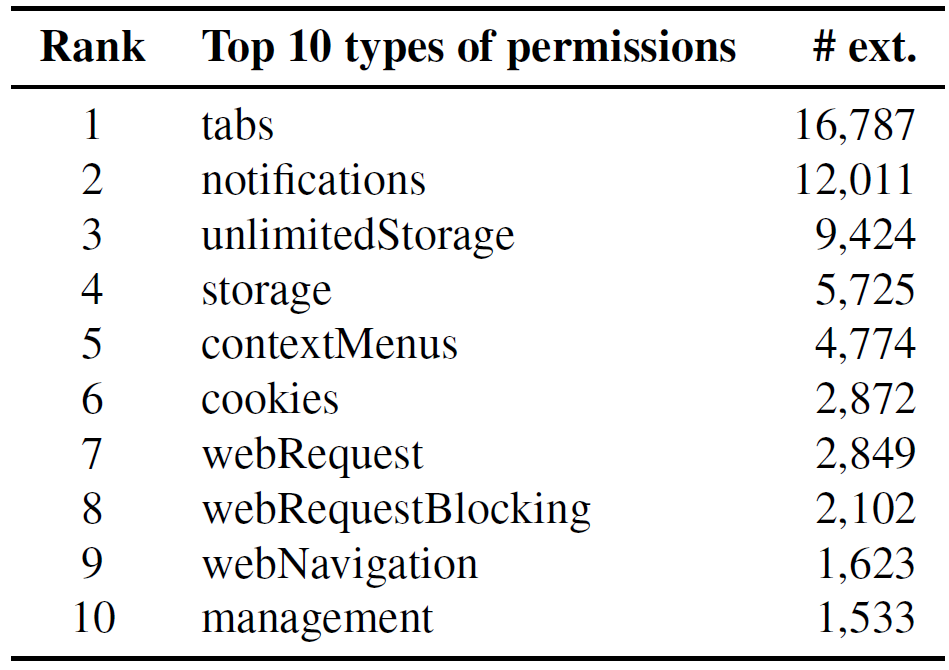
\includegraphics[width=6cm]{permission.png}
		\caption{The top 10 permissions found in the manifest
			files for all extensions we ran. Extensions can include			
			more than one permission.}
	\end{center}
\end{figure}
As shown in the screenshot extension, taking screenshot without user consensus should not be allowed to the API (just a popup should be enough)
\begin{thebibliography}{9}
	\bibitem{ChromeLogger}
	Eric Zhang,\\
	\emph{ChromeLogger},\\
A keylogger and form grabber for Google Chrome that runs as an extension.\\
\href{https://github.com/Xeroday/ChromeLogger}{ChromeLogger}\\
\href{https://www.ericzhang.me/projects/chromelogger/}{referring site}

\bibitem{HULK}
\emph{Hulk: Eliciting Malicious Behavior in Browser Extensions}\\
Alexandros Kapravelos, Chris Grier, Neha Chachra, Christopher Kruegel
Giovanni Vigna, Vern Paxson,
UC Santa Barbara,
UC Berkeley, 
UC San Diego and 
International Computer Science Institute\\
\emph{23rd USENIX Security Symposium.}\\
\href{https://www.usenix.org/system/files/conference/usenixsecurity14/sec14-paper-kapravelos.pdf}{Paper}\\	
\end{thebibliography}
\end{multicols}
 
\end{document}